\let\negmedspace\undefined
\let\negthickspace\undefined
\documentclass{scrreprt}
\usepackage[a5paper, margin=10mm, onecolumn]{geometry}
\usepackage{lmodern} 
\usepackage{tfrupee} 
\setlength{\headheight}{1cm}
\setlength{\headsep}{0mm}   

\usepackage{gvv-book}
\usepackage{gvv}
\usepackage{cite}
\usepackage{amsmath,amssymb,amsfonts,amsthm}
\usepackage{algorithmic}
\usepackage{graphicx}
\usepackage{textcomp}
\usepackage{xcolor}
\usepackage{txfonts}
\usepackage{listings}
\usepackage{enumitem}
\usepackage{mathtools}
\usepackage{gensymb}
\usepackage{comment}
\usepackage[breaklinks=true]{hyperref}
\usepackage{tkz-euclide} 
\usepackage{listings}                             
\def\inputGnumericTable{}                                 
\usepackage[latin1]{inputenc}                                
\usepackage{color}                                            
\usepackage{array}                                            
\usepackage{longtable}                                       
\usepackage{calc}                                             
\usepackage{multirow}                                         
\usepackage{hhline}                                           
\usepackage{ifthen}                                           
\usepackage{lscape}
\usepackage{xparse}
\usepackage{multicol}

\bibliographystyle{IEEEtran}

\title{UGV-UAV}
\author{Jnanesh Sathisha Karmar\\Vivek K Kumar}

\begin{document}
\maketitle

\renewcommand{\thefigure}{\theenumi}
\renewcommand{\thetable}{\theenumi}

\numberwithin{equation}{enumi}
\numberwithin{figure}{enumi} 

\tableofcontents

\chapter{Introduction}
\section{Motivation \& Objective}
To integrate UAV architecture into UGV and have a unified control system for both ecosystems. This is efficient, and also enables for the testing of UAVs through UGVs, as effectively UAVs only have an extra dimension.

\chapter{Unmanned Aerial Vehicle (UAV)}
\section{The Brain: ArduPilot Flight Controller}
ArduPilot is a versatile autopilot system for \textbf{Multicopters, Rovers, Boats, and Planes}. It reads sensors (Gyro, GPS)  to controls motors. One of the most important advantages of this is that it handles both high-speed flight stabilization and precise ground steering. 

\bigskip
\resizebox{0.9\columnwidth}{!}{
\begin{tikzpicture}[
    node distance=2cm,
    auto,
    block/.style={
        rectangle,
        draw,
        fill=cyan!10,
        text width=1.5cm,
        text centered,
        rounded corners,
        minimum height=3em,
        line width=0.8pt
    },
    line/.style={
        draw,
        -latex,
        thick,
        color=blue!70!black
    },
    power/.style={
        draw,
        -latex,
        dashed,
        thick,
        color=red!70!black
    }
]

    % Components
    \node [block] (fc) {ArduPilot Flight Controller};
    \node [block, above=1.5cm of fc] (compass) {Compass (Nav)};
    \node [block, below=1.5cm of fc] (batt) {12.6V Battery};
    \node [block, right=2cm of fc] (esc) {ESC};
    \node [block, right=1.5cm of esc] (motor) {Drone Motors};
    \node [block, right=1.5cm of motor] (prop) {Propellers};

    % Signal/Data Connections (Blue Solid)
    \path [line] (compass) -- node[pos=0.5, left, font=\footnotesize] {Heading Data} (fc);
    \path [line] (fc) -- node[pos=0.5, above, font=\footnotesize] {PWM Signal} (esc);
    \path [line] (esc) -- node[pos=0.5, above, font=\footnotesize] {3-Phase AC} (motor);
    \path [line] (motor) -- node[pos=0.5, above, font=\footnotesize] {Torque} (prop);

    % Power Connections (Red Dashed)
    \path [power] (batt) -- node[pos=0.5, left, font=\footnotesize] {DC Power} (fc);
    \path [power] (batt) -| node[pos=0.2, below, font=\footnotesize] {High Current DC} (esc);

\end{tikzpicture}
}

\subsection{How to load firmware}
We do not have to write C++ code from scratch to run the microcontroller. Precompiled firmware is available in the \hyperlink{https://ardupilot.org/}{ArduPilot website}, from which Flash specific stacks (e.g., ArduCopter/ArduRover) can be flashed into ArduPilot via Mission Planner.
Mission Planner can also be used to fix the initial parameters(e.g., Radio calibration, ESC calibration) to get the UAV ready for flight.

\subsection{Mission Planner}
Mission Planner is a free, open-source Ground Control Station (GCS) software used to configure, monitor, and control autonomous vehicles such as drones, planes, rovers, and boats that run on ArduPilot firmware. It provides a graphical interface to communicate with the flight controller through USB or telemetry radios. Mission Planner allows users to upload flight missions, set waypoints, tune parameters, calibrate sensors, and monitor real-time flight data such as altitude, speed, GPS position, and battery status.
\begin{figure}[H]
    \centering
    
\includegraphics[width=0.8\linewidth]{figs/Mission planner.png}
    \caption{Mission Planner interface}
    \label{fig:placeholder}
\end{figure}
\chapter{Dabble}
Dabble is a mobile application developed by STEMpedia that enables smartphones to function as wireless controllers for microcontroller-based systems such as Arduino, ESP32, and other embedded platforms. It uses Bluetooth communication to connect the smartphone with the hardware, allowing users to control, monitor, and interact with electronic projects in real time.
Dabble provides a set of pre-built modules that simplify interfacing between hardware and smartphone sensors, eliminating the need to design complex mobile applications from scratch. Through its graphical interface, users can access smartphone features such as buttons, sensors, camera input, and motion detection, and transmit that data directly to the microcontroller.

\section{Component Architecture with Dabble}
\resizebox{\textwidth}{!}{%
\begin{tikzpicture}[
    node distance=1.2cm and 1.2cm, % Reduced spacing for better fit
    auto,
    block/.style={
        rectangle,
        draw,
        fill=cyan!10,
        text width=2.5cm,
        text centered,
        rounded corners,
        minimum height=3em,
        line width=0.8pt
    },
    line/.style={
        draw,
        -latex,
        thick,
        color=blue!70!black
    },
    wireless/.style={
        draw,
        -latex,
        thick,
        dashed,
        color=blue!70!black
    },
    power/.style={
        draw,
        -latex,
        dashed,
        thick,
        color=red!70!black
    }
]

    % --- Nodes ---
    
    % Top Row
    \node [block] (esp) {ESP32 Controller};
    \node [block, left=of esp] (phone) {Smartphone \\ (Dabble App)};

    % Bottom Row
    % Key Change: Place Battery directly BELOW the ESP32 to simplify wiring
    \node [block, below=2cm of esp] (batt) {Battery Source};
    
    % Place Driver to the RIGHT of Battery
    \node [block, right=of batt] (driver) {L298N Driver};
    
    % Place Motors/Wheels extending to the right
    \node [block, right=of driver] (motor) {4x DC Motors};
    \node [block, right=of motor] (wheel) {Wheels};

    % --- Connections ---
    
    % 1. Bluetooth (Top Left)
    \path [wireless] (phone) -- node[above, font=\footnotesize] {Bluetooth} (esp);

    % 2. Logic Power (Straight Up)
    \path [power] (batt) -- node[left, font=\footnotesize, align=right] {Logic\\Power} (esp);

    % 3. Motor Power (Straight Right)
    \path [power] (batt) -- node[above, font=\footnotesize] {Motor Power} (driver);

    % 4. GPIO/PWM Control (Right then Down)
    % Uses -| to go Horizontal from ESP, then Vertical down to Driver
    \path [line] (esp) -| node[pos=0.2, above, font=\footnotesize] {GPIO/PWM} (driver);

    % 5. Drive & Torque
    \path [line] (driver) -- node[above, font=\footnotesize] {DC Drive} (motor);
    \path [line] (motor) -- node[above, font=\footnotesize] {Torque} (wheel);

\end{tikzpicture}
}

\section{Controlling Ground Vehicle with Dabble}


\textbf{Setup \& Connection:}
\begin{enumerate}
    \item Install \textbf{Dabble} app (Android).
    \item Enable Bluetooth on your phone.
    \item Open the app and select the \textbf{Gamepad} module.
    \item Tap the \textbf{Plug Icon} (Connect) at the top right.
    \item Select your ESP32 (e.g., \textit{"JNANU"}).
\end{enumerate}

\vspace{0.3cm}
\textbf{Controls:}
\begin{itemize}
    \item Use the \textbf{Digital Mode} (Arrow keys).
    \item \textbf{Up/Down:} Move Forward/Backward.
    \item \textbf{Left/Right:} Turn (Differential Drive).
\end{itemize}

\begin{figure}[H]
\centering

\includegraphics[width=\textwidth, height=0.8\textheight, keepaspectratio]{figs/dabble.png}
\vspace{0.2cm}
\footnotesize \textit{Dabble Gamepad Interface}
\end{figure}


\chapter{FLYSKY Remote}
The Flysky FS-i6 is a 2.4 GHz wireless radio transmitter used for remote control of electronic systems such as drones, robots, RC cars, airplanes, and embedded systems. It is part of the Flysky radio control ecosystem and works together with compatible receivers (such as FS-iA6 or FS-iA6B) to transmit user commands wirelessly to a microcontroller or motor control system.The FS-i6 converts physical inputs from joysticks, switches, and knobs into digital signals, which are transmitted using the AFHDS 2A (Automatic Frequency Hopping Digital System) protocol. The receiver connected to the robot or vehicle interprets these signals and sends corresponding control signals to motors, servos, or microcontrollers.
\begin{figure}[H]
    \centering
    
\includegraphics[width=0.5\linewidth]{figs/flysky.jpg}
    \caption{flysky remote}
    \label{fig:placeholder}
\end{figure}
\section{Component Architecture in UGV (FlySky)}
\begin{tikzpicture}[
    node distance=1.5cm and 1.2cm,
    auto,
    block/.style={
        rectangle,
        draw,
        fill=cyan!10,
        text width=1.3cm,
        text centered,
        rounded corners,
        minimum height=3em,
        line width=0.8pt
    },
    line/.style={
        draw,
        -latex,
        thick,
        color=blue!70!black
    },
    wireless/.style={
        draw,
        -latex,
        thick,
        dashed,
        color=blue!70!black
    },
    power/.style={
        draw,
        -latex,
        dashed,
        thick,
        color=red!70!black
    }
]

    % --- Top Row: Control Flow ---
    \node [block] (esp) {ESP32 Controller};
    \node [block, left=of esp] (rx) {Receiver \\ (FS-iA6B)};
    \node [block, left=of rx] (tx) {FlySky \\ Transmitter};

    % --- Bottom Row: Power & Drive ---
    % Align Driver below ESP32
    \node [block, below=2cm of esp] (driver) {L298N Driver};
    % Align Battery below Receiver
    \node [block, below=2cm of rx] (batt) {Battery Source};
    
    % Motors and Wheels to the right
    \node [block, right=of driver] (motor) {4x DC Motors};
    \node [block, right=of motor] (wheel) {Wheels};

    % --- Connections ---

    % 1. Wireless Control (Tx -> Rx)
    \path [wireless] (tx) -- node[above, font=\footnotesize] {2.4GHz} (rx);

    % 2. Receiver Signal (Rx -> ESP32)
    \path [line] (rx) -- node[above, font=\footnotesize] {Pulse} (esp);

    % 3. Motor Control (ESP32 -> Driver)
    \path [line] (esp) -- node[right, font=\footnotesize] {GPIO / PWM} (driver);

    % 4. Power Distribution
    % Battery -> Driver (Motor Power)
    \path [power] (batt) -- node[above, font=\footnotesize] {Motor Power} (driver);
    
    % Battery -> ESP32 (Logic Power) - Path goes Up then Right
    \path [power] (batt) -- node[sloped, above, font=\footnotesize] {Logic Power} (esp);
    
    % Battery -> Receiver (Optional explicit power line, or simplified via ESP)
    % Here we show a small branch for Rx power for completeness
    \path [power] (batt) -- (rx); 

    % 5. Drive Output
    \path [line] (driver) -- node[above, font=\footnotesize] {DC Drive} (motor);
    \path [line] (motor) -- node[above, font=\footnotesize] {Torque} (wheel);

\end{tikzpicture}

\chapter{Operating UGV through ArduPilot}
\section{Integration with L298N Motor Drivers}

\begin{figure}[H]
    \centering
    
\includegraphics[width=0.4\linewidth]{figs/l298n.png}
    \caption{L298N}
    \label{fig:l298n}
\end{figure}

The system architecture follows a sequential control flow from the APM 2.8 flight controller, through an ESP32 microcontroller, to an L298N motor driver, which ultimately powers the DC motors. A direct connection between the APM and the motor driver is unfeasible due to a fundamental signal mismatch. Specifically, the APM 2.8 outputs standard RC servo PWM pulses ranging from 1000~$\mu$s to 2000~$\mu$s, whereas the L298N driver requires logic-level directional inputs (HIGH/LOW) and standard duty-cycle PWM (0--100\%) to regulate speed. To bridge this gap, the ESP32 functions as a dedicated signal translator. It continuously reads the incoming pulse widths from the APM's throttle and steering outputs and mathematically maps these values to the required motor driver formats. For example, the ESP32 is programmed to interpret a signal of 1000--1450~$\mu$s as a reverse command, 1450--1550~$\mu$s as a neutral deadband for stopping or braking, and 1550--2000~$\mu$s as forward motion. Based on this real-time mapping, the ESP32 drives the appropriate pins on the L298N to achieve precise locomotion.

\subsection{Setup}
\begin{enumerate}
    \item Install ArduRover v2.5.1 firmware in mission planner for APM 2.8
    \item Calibrate radio, compass, GPS, accelerometer and servo output in Mission Planner
    \item Wire APM 2.8 as follows:
    \begin{itemize}
        \item Inputs: Connect radio receiver and GPS/Compass module. Also power it up through the 5V L298N motor driver line.
        \item Outputs: Connect signal lines of 1 and 3 to ESP32. 
    \end{itemize}
    \item Upload the code into the ESP32. The code is available here\\
        \fbox{\parbox{\linewidth}{\url{https://github.com/Vivek-Kumar-1907/uavugv/blob/main/codes/main.ino}
}}
\end{enumerate}

\subsection{Result}
We have hence successfully translated the entire UAV architecture into UGV architecture.


\end{document}  
